\documentclass[oneside]{book}
\usepackage[utf8]{inputenc}
\usepackage{authblk}
\usepackage{setspace} 
\usepackage{amsmath}
\usepackage{textcomp}
\usepackage{amssymb}
\usepackage{geometry}
\usepackage{amsthm}
\usepackage{runic}
\usepackage{mathtools}
\usepackage{graphicx}
\usepackage[breaklinks=true,a4paper=true,pagebackref=true]{hyperref}
\graphicspath{ {figures/} }
\geometry{
 a4paper,
 total={170mm,257mm},
 left=20mm,
 top=20mm,
}
\hypersetup{
    colorlinks=true,
    linktoc=true,
    linkcolor=blue,
}
\title{Libraria Algebrae}
\author{Liam Gardner}
\date{\today}
%\doublespacing
\newcommand\tab[1][1cm]{\hspace*{#1}}
\newcommand\nextline{\newline\tab}
\newcommand\nextquestion{\newline\newline}
\newcommand\soln{$\text{sol}^\text{n}\text{ }$}
\newcommand\fs{\mbox{\large $\mathrlap{f}s\,$}\,}
\newcommand\thm[2]{\section*{Theorem: #1}\label{sec:#2}\addcontentsline{toc}{section}{Theorem: #1}}
\newcommand\propn[2]{\section*{Proposition: #1}\label{sec:#2}\addcontentsline{toc}{section}{Proposition: #1}}
\newcommand\defn{\textbf{Definition}: }

\renewcommand\mod[1]{\text{ }\left(\text{mod }#1\right)}


\begin{document}
\DeclarePairedDelimiter\abs{\lvert}{\rvert}

\maketitle
\tableofcontents
\chapter{Linear Diophantine Equations in $\mathbb{Z}^2$}
\tab
Note that for the general equation $ax+by$, we assume that $ab\neq0$, since if one is 0, then the equation is trivial. We wish to answer three fundamental problems
\begin{enumerate}
\item Does there exist an integer solution?
\item If the answer is yes, find an integer solution.
\item Can we find \textit{all} solutions?
\end{enumerate}
\tab
It is common for existential theorems (those that say solutions exist) to not give a means of how to find said solutions.
\subsection{Example}
Solve $506x + 391y = 23$. Notice that $\gcd(506,391)=23$. Thus, by b\'ezout's\ lemma, a solution exists. We can use the EEA (Extended Euclidean Algorithm) to find a solution to the equation. 
\newline
\begin{center}
\begin{tabular}{|c|c|c|c|}
\hline
$x$ & $y$ & $r$ & $q$ \\
\hline
\hline
1 & 0 & 506 & 0 \\
0 & 1 & 391 & 0 \\
1 & -1 & 115 & 1.0 \\
-3 & 4 & 46 & 3.0 \\
7 & -9 & 23 & 2.0 \\
-17 & 22 & 0 & 2.0 \\
\hline
\end{tabular}
\end{center}
\tab
Thus, we know that $(7,-9)$ is a solution. Now, we can subtract the equation $506x+391y=23$ with $506x_0 + 391y_0=23$, which gives $506(x-x_0) + 391(y-y_0) = 0$. Thus, we get $506(x-x_0) = -391(y-y_0)$. We can divide by the GCD of 506 and 391 to get the equation $22(x-x_0) = -17(y-y_0)$. Since the GCD is a common divisor to 506 and 391, we get that both $\frac{506}{23}$ and $\frac{391}{23}$ are integers and are coprime to each other. Now, since we know that $-17\lvert -17(y-y_0)$, and that $-17(y-y_0)=22(x-x_0)$, we get that $-17\lvert 22(x-x_0)$. Thus, by CAD, we get $17\lvert (x-x_0)$. Therefore, we find that $x-x_0 = 17n$ for some $n\in\mathbb{Z}$. Thus, a solution for $x$ can be found with $x_0 + 17n$, $\forall n\in\mathbb{Z}$.
\nextline
Following the same process, we get that $y=y_0+22n$. Therefore, all solutions to the Linear Diophantine Equation $506x + 391y = 23$ are given by the points $(7 + 17n, -9 - 22n)$.
\newline
\newline
Solve $506x + 391y = 24$.
\nextline
There are no \soln: Since $23=\gcd(506,391)$, we get that $23\lvert 506x+391y$ however, $23\nmid 24$, therefore, we've run into a contradiction.
\newline
\newline
Solve $506x + 391y = 46 = 2\cdot23$. We know that $506\cdot7 + 391\cdot(-9) = 23$, thus if we multiply both sides by two, we get that $506(7\cdot2) + 391(-9\cdot2) = 2\cdot23 = 46$. $506(14) + 391(-18) = 46$ gives the \soln (14,-18).

\thm{LDET Part 1}{ldeta}

Suppose $a,b,c\in\mathbb{Z}$ and $ab\neq0$ then $ax+by=c$ has a \soln in integers if and only if $\gcd(a,b)\lvert c$.
\subsection{Proof of forwards direction}
\tab
Assume $ax+by=c$ has an integer \soln $(x_0, y_0)$. Let $d=\gcd(a,b)$. Since $d\lvert a$ and $d\lvert b$, and since $c=ax_0+by_0$, then by Divsibility of Integer Combinations, $d\lvert c$.
\subsection{Proof of backwards direction}
\tab
Let $d=\gcd(a,b)$, and assume that $d\lvert c$, thus $c=kd$ \fs integer $k$. Then By B\'ezout's\ Lemma, we can find $x_0$ and $y_0$ $\in\mathbb{Z}$ such that $ax_0+by_0=d$, but then $k(ax_0+by_0)=kd$. Thus $a(kx_0) + b(ky_0) = c$
\subsection{Remark}
\tab
if $d\lvert c$ then the proof tells us how to find a \soln.
\begin{enumerate}
\item solve $ax+by=d$ using EEA to get $(x,y)=(x_0,y_0)$.
\item take $x=kx_0$ and $y=ky_0$, where $k=\frac{c}{d}$.
\end{enumerate}

\thm{LDET Part 2}{ldetb}

Suppose that $(x_0, y_0)$ is a particular solution to the LDE $ax+by=c$.
\nextline
Then the set of all \soln $\in\mathbb{Z}$ is given by the following set:
$$S = \left\{
(x,y) \Huge\mid x=x_0 + \frac{b\cdot n}{\gcd(a,b)},\,\,\, y=y_0 - \frac{a\cdot n}{\gcd(a,b)}
\right\}$$
\subsection{Proof}
\tab
Let $D$ be the set of all integer solutions to $ax+by=c$. I.E.
$$D = \left\{(x,y) \mid x,y,\in\mathbb{Z}, ax+by=c \right\}$$
\tab
This can be proven by showing $S \subseteq D$ and $D \subseteq S$
\newline $S\subseteq D:$
\nextline
Let $(x,y) \in S$, thus $x=x_0 + \frac{bn}{d}$ and $y=y_0-\frac{an}{d}$.
$$ax+by = a\left(x_0+\frac{bn}{d}\right) + b\left(y_0 - \frac{an}{d}\right)$$
$$= ax_0 + by_0 = c$$
\tab
since by definition, we know that $x_0$ and $y_0$ are a particular solution to the equation. Therefore, $S\subseteq D$
\newline $D\subseteq S:$
\nextline
Let $(x,y)\in D$, thus $x,y\in\mathbb{Z}$ and $ax+by=c$. Since, $(x_0,y_0)\in D$, we know that $ax_0 + by_0 = c$. We can subtract $ax_0+by_0=c$ from $ax + by = c$ to get $a(x-x_0) + b(y-y_0) = 0$. Dividing by the GCD of $a$ and $b$, we get that $\frac{a(x-x_0)}{d} = \frac{-b(y-y_0)}{d}$. Thus, since $\frac{b}{d}\lvert \frac{a}{d}(x-x_0)$ then by CAD, we get that $\frac{b}{d}\lvert (x-x_0)$, since $\frac{b}{d}$ and $\frac{a}{d}$ are coprime. Then we get $x-x_0=n\frac{b}{d}\Rightarrow x=x_0+\frac{bn}{d}$ \fs $n\in\mathbb{Z}$. Similarly, we get $y=y_0-\frac{an}{d}$. Therfore, $(x,y)\in S$.
\section{More Examples}
$12x+18y=13$.
\nextline
$\gcd(12,18) = 6$. Since $6\nmid13$ the equation has no \soln by \hyperref[sec:ldeta]{LDET1}
\newline
\newline
$14x-49y=28$
\nextline
$\gcd(14,-49) = 7$. Since $7\lvert 28$ the equation has solutions by \hyperref[sec:ldetb]{LDET2}
\nextline
Consider $14x-49y=7\Rightarrow 2x-7y=1$ which has \soln $(4,1)$. If we multiply $14(4) - 49(1) = 7$ by 4, we get that $14(x_0\cdot4) - 49(y_0\cdot4) = 7$, and from this we can get all \soln using LDET2.
\newline
\newline
\tab
Find all \soln to $15x+35=5$.
\newline
\begin{center}
\begin{tabular}{|c|c|c|c|}
\hline
$x$ & $y$ & $r$ & $q$ \\
\hline
\hline
1 & 0 & 15 & 0 \\
0 & 1 & 35 & 0 \\
1 & 0 & 15 & 0.0 \\
-2 & 1 & 5 & 2.0 \\
7 & -3 & 0 & 3.0 \\
\hline
\end{tabular}
\end{center}
\tab
Thus, we know that $\gcd(15,35)=5$, and $5\lvert 5$, there is a \soln. By EEA, we find $x=-2, y=1$ is a \soln. Then, we can find the general solution using
\hyperref[sec:ldetb]{LDET2}
 to be $x=-2+\frac{35n}{5}\Rightarrow 7n-2$, $y=1+\frac{15n}{5}\Rightarrow 1+3n$
\subsection{Geometric Understanding}
\tab
Graphing the line $15x+35y=5$ or $3x+7y=1$, we can rearrange for $y$ to get $y=\frac{-3}{7}x+\frac{1}{7}$. Thus, picking any lattice point, we can construct a triangle of length 7 and height 3 from that point to find the next lattice point.

\begin{figure}[h]
\centering
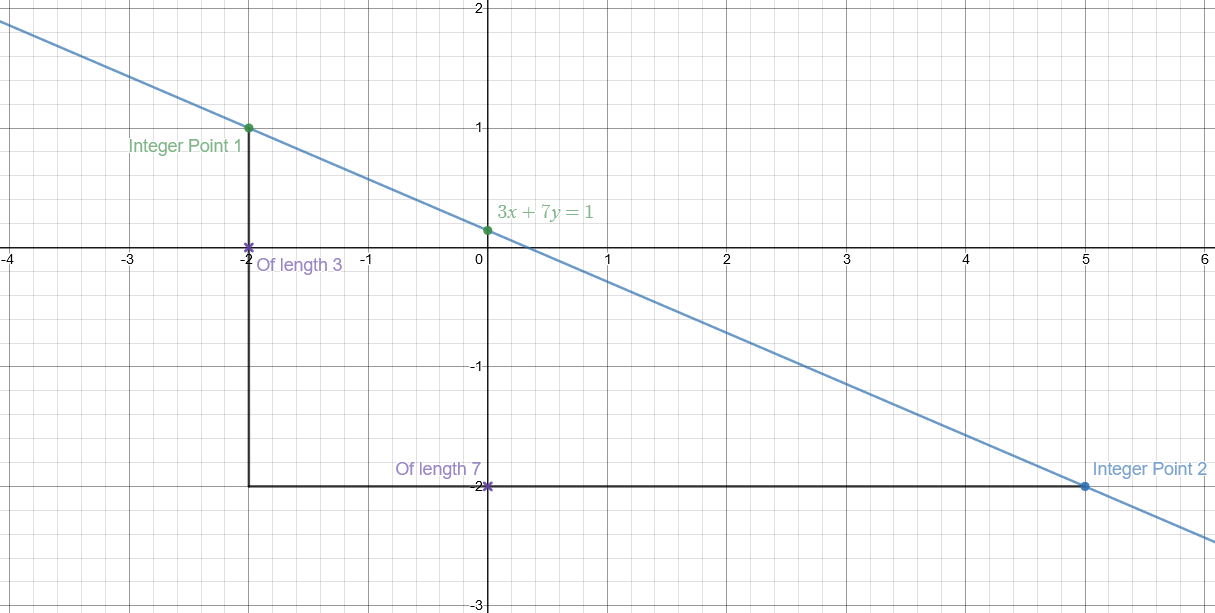
\includegraphics[width=0.5\textwidth]{l24f0}
\caption{Triangle formed from moving between two lattice points}
\end{figure}

\subsection{Nonnegative \soln}
\tab
The solutions to $15x+35y=5$ is given by $(-2+7n, 1-3n)$, these will be nonnegative if $x\geq0$ and $y\geq0$.
$$-2+7n\geq 0 \iff n\geq \frac{2}{7}$$
$$1-3n \geq 0 \iff n \leq \frac{1}{3}$$
Thus, since there are no integer solutions in the range $\frac{2}{7}\leq n \leq \frac{1}{3}$, as $n\in\mathbb{Z}$ there are no nonnegative solutions.
\subsection{Find all integer \soln to $15x+35y^2 = 5$}
\tab
Let $Y=y^2$, then, since we have the \soln to $15x+35Y=5$, given by $(-2+7n, 1-3n)$, all we have to do is see when $1-3n$ is a perfect square.
One way to solve this is to say let $z=y^2$ and solve $1-3n=z$. We can also solve this algebraically
\newline
\begin{center}
\begin{tabular}{c c c}
$\iff$ & $1-3n = y^2$ & \\
$\iff$ & $-3n=y^2-1$ & \\
$\iff$ & $3\lvert y^2-1$ & by euclid's lemma \\
$\iff$ & $3\lvert(y-1)(y+1)$ & \\
\end{tabular}
\end{center}
\tab
By Euclid's Lemma, we know either $3\lvert(y-1)$ or $3\lvert(y+1)$, though not both. Suppose $3\lvert(y-1) \iff y-1=3k\iff y=3k+1\, \fs k\in\mathbb{Z}$
Then, if $y=3k+1$, we get that $y^2=(1+3k)^2=1-3(-2k-3k^2)$. Let $n=(-2k-3k^2)$, then we get $y^2=1-3n$. Thus, if we take $x=-2+7n=-2+7(-2-3k^2)$ and $y=1-3k$, we get a perfect square \soln to the diophantine equation. 
\nextline
If $3\lvert y+1$, then we have $y=-1+3l\, \fs l \in \mathbb{Z}$. Then $y^2=(-1+3l)^2=1-3(2l+3l^2)$. Thus, $y=1-3l$ and $x=-2+7(2l+3l^2)$. Therfore, we can generate infinitely many perfect square solutions.
\chapter{Congruence and Modular Arithmetic}
\section{Clockwork Arithmetic Analogy}
\tab
Imagine a clock, we know that a clock has 12 spokes. If we look at it and see the hour hand at 2, and we know that 12 has already passed, then we also know that the clock really means it's 14. Thus, we can say $2\approx14$
\section{Definition}
\tab
$\forall a,b\in\mathbb{Z}$, we say that ``$a$ is congruent to $b$ mod(ulo) 12'' if $m\lvert(a-b)$.
\nextline
Notation: $a\equiv b\mod{m}$
\section{Examples}
\tab
$m=1$ then $a\equiv b\mod{1} \iff 1\lvert (a-b)$ which is true $\forall a,b\in\mathbb{Z}$
\nextline
$m=2$ then $a\equiv b\mod{2} \iff 2\lvert (a-b) \iff a-b$ is even $\iff a$ and $b$ are both even or both odd.
\nextline
$2\equiv-116\mod{2}$, however $3\not\equiv 10024\mod{2}$
\nextline
$14\equiv 2\mod{12} \iff 12\lvert(14-2)$
\nextline
$6\equiv 26\mod{10} \iff 10\lvert(6-26)$
\nextline
$6\not\equiv -26\mod{10} \implies 10\nmid(6+26)$
\propn{Congruence is an Equivalence Relation}{CER}
\begin{center}
\begin{tabular}{l|l}
$\forall m\in\mathbb{N}, \forall a,b,c,\in\mathbb{Z}$ & Congruence is \\
\hline
\hline
$a\equiv a\mod{m}$ & symmetric \\
if $a\equiv b\mod{m}$ and $b\equiv c\mod{m}$ then $a\equiv c\mod{m}$ & transitive \\
$a\equiv b \mod{m}\implies b\equiv a\mod{m}$ & Reflexive
\end{tabular}
\end{center}
\tab
Remark: Any relation $a\sim b$ that satisfies all above properties is called an equivalence relation.
\nextline
In calculus, we say two functions $f(x)\sim g(x)$ are an equivalence relation if $f^\prime(x) = g^\prime(x)$
\section{Recap}
\tab
Fix $m\in\mathbb{N}$, $\forall a,b\in\mathbb{Z}$
\nextline
\begin{tabular}{l c l}
$a\equiv b\mod{m}$ & $\iff$ & $m\lvert (a-b)$ \\
& $\iff$ & $a-b=mk\,\, \fs k\in\mathbb{Z}$ \\
& $\iff$ & $a=b+mk$
\end{tabular}
\newline
\propn{Arithmetic Rules of Congruence}{ARC}
Suppose $a\equiv a^\prime \mod{m}$ and $b\equiv b^\prime \mod{m}$ then,
\begin{enumerate}
\item $a+b\equiv a^\prime + b^\prime \mod{m}$
\item $a-b\equiv a^\prime - b^\prime \mod{m}$
\item $ab\equiv a^\prime b^\prime \mod{m}$
\end{enumerate}
\subsection{Examples}
$$2\equiv 9\mod{7}\land3\equiv 17\mod{7}\implies 2+3\equiv9+17\mod{7}\implies 5=26$$
\newline
$$56\cdot30 \mod{40}$$
$$56=16+40\equiv 16\mod{40}$$
$$30=-10\equiv \mod{40}$$
$$56\cdot30 \equiv 16\cdot(-10)\mod{40}$$
$$\equiv-160\mod{40}$$
$$\equiv-40\cdot4\mod{40}\equiv 0\mod{40}$$
\subsection{Proof of addition}
\tab
Since $a\equiv a^\prime \mod{m}$ and $b\equiv b^\prime \mod{m}$ then $m\lvert(a-a^\prime)$ and $m\lvert(b-b^\prime)$
\nextline
We have $(a+b)-(a^\prime-b^\prime)=a-a^\prime + b-b^\prime$, thus by DIC we get $m\lvert((a+b)-(a^\prime+b^\prime))$. Therefore $a+b\equiv a^\prime + b^\prime \mod{m}$
\subsection{Remark on Division}
\tab Care is needed with division
$ab\equiv ac\mod{m} \not\implies b\equiv c\mod{m}$ even if $a\not\equiv 0 \mod{m}$
\nextline
$$10\equiv 4\mod{6}$$
$$2\cdot5 \equiv 2\cdot2 \mod{6}$$
$$5\not\equiv 2\mod{6}$$
\propn{Congruent Division}{CD}
\tab
If $ab\equiv ac\mod{m}$ and $a$ is coprime to $m$, then $b\equiv c\mod{m}$
\propn{Congruent Powers}{CP}
\tab
$a\equiv b\mod{m}\implies a^n\equiv b^n\mod{m}$
\subsection{Proof}
\tab
$$ab\equiv bc\mod{m}\iff m\lvert (ab-ac)\iff m\lvert a(b-c)$$
\nextline
Then by CAD we get $m\lvert(b-c)$ since $m$ and $a$ are coprime\nextline
$\implies b\equiv c \mod{m}$
\nextline
By applying the above proposition repeatedly; if $a_1\equiv a^\prime_1 \mod{m}, a_2\equiv a^\prime_2 \mod{m}, \cdots a_n\equiv a^\prime_n \mod{m}$, then we get the following result
\begin{enumerate}
\item $a_1+\cdots+a_n\equiv a^\prime_1 + \cdots a^\prime_n \mod{m}$
\item $a_1-\cdots-a_n\equiv a^\prime_1 - \cdots a^\prime_n \mod{m}$
\item $a_1\cdots a_n\equiv a^\prime_1 \cdots a^\prime_n \mod{m}$
\item (special case) $\forall q \in \mathbb{N}, a^q \equiv \left(a^\prime\right)^q \mod{m}$
\end{enumerate}
\subsection{More Examples}
Simplify $4^10 \mod{18}$\nextline
$4^{10} = \left(4^2\right)^5 = 16^5=(18-2)^5$ \nextline
$(18-2)^5\equiv-2^5\mod{18}$ \nextline
$\equiv-32\mod{18}$ \nextline
$-32+2\cdot 18\mod{18}$ \nextline
$4\mod{18}$
\newline
\newline
Is $3^9 + 62^{2020} - 20$ divisible by 7?
\nextline
Let $n=3^9+62^{2020}-20$. We know that $7\lvert n \iff 7\lvert(n-0) \iff n\equiv0\mod{7}$
\nextline
We can compute $3^9=\left(3^3\right)^3=27^3=(28-1)^3$ \nextline
$\equiv (-1)^3\mod{7}$\nextline
$\equiv -1\mod{7}$\nextline
We also know that $62^{2020} = (63-1)^{2020} \equiv (-1)^{2020}\mod{7} \equiv 1$ \nextline
$20=21-1\equiv -1\mod{7}$ \nextline
Using \hyperref[sec:ARC]{The arithmetic rules} we get that $n\equiv -1+1-(-1)\mod{7}\equiv1\mod{7}$ and thus $n$ is not divisible by 7.
\thm{Congruence and Remainders}{CR}
\subsection{Example}
\tab
What day of the week is it going to be a year from now?
\nextline
Since days cycle every 7, let's determine $365\mod{7}$. We know that $350=50\cdot7$ and thus \nextline $365 = 350 + 15$ \nextline
$=7\cdot50+14+1$ \nextline
$=7\cdot50+7\cdot2+1$\nextline
$=7(50+2)+1$\nextline
$\equiv 1\mod{7}$.\nextline
$365\equiv1\mod{7}$\nextline
Therefore, the day of the week one year from now is the same as the day of the week tomorrow.
\subsection{Observation}
\tab
if $n\in\mathbb{Z}$ \nextline
Any block of consecutive numbers will cycle through the numbers 0-6 inclusive:
$$\{\cdots,-7,-6,-5,-4,-3,-2,-1,0,1,2,3,4,5,6,7,8,9,10,11,12,13,14,\cdots\}$$
$$\equiv\{\cdots,0,1,2,3,4,5,6,0,1,2,3,4,5,6,0,1,2,3,4,5,6,\cdots\}\mod{7}$$
\section{Warning}
\tab
$\forall a,b,b^\prime \in \mathbb{N}$, if $b\equiv b^\prime \mod{m}$ then in general $a^b\not\equiv a^{b^\prime}\mod{m}$
\subsection{Example}
\tab
$4\equiv1\mod{3}$\nextline
$2^4=16\equiv1\mod{3}$ however $2^1\equiv 2\mod{3}$ \nextline
Thus $4\equiv1\mod{3}$ however $2^4\not\equiv2^1\mod{3}$
\propn{Finite Integers}{FI}
$\forall a,b,\in\mathbb{Z} a\equiv b \mod{m}\iff a$ and $b$ have the same remainder after division by $m$
\subsection{Proof}
\tab
Applying the division algorithm, we get $a=qm+b$ and $b=q^\prime m+r^\prime$ where $0\leq r,r^\prime < m$.\nextline
Notice if $a\equiv b\mod{m}$, we get that $m\lvert(a-b)$ and thus $m\lvert(qm+r - q^\prime m - r^\prime)$\nextline
$\implies m\lvert(m(q+q^\prime) + (r-r^\prime))$ Then by DIC it follows that \nextline
$\iff m\lvert (r-r^\prime)$ \nextline
Now since $0\leq r < m$ and $0 \leq r^\prime < m$, we get that $-m\leq r-r^\prime < m$. Now, since $m\lvert(r-r^\prime)$, we get that by BBD, that $m\leq \abs{r-r^\prime}$ and so for both inequalities to hold, $r=r^\prime$.
\propn{Congruent if and only if same remainder}{CISR}
\tab
$a\equiv b\mod{m} \iff a$ and $b$ have the same remainder after division by $m$.
\propn{Congruent to Remainder}{CTR}
$\forall a,b\in\mathbb{Z}\,, 0\leq b \leq m-1 : a\equiv b\mod{m}\iff$ the remainder of $a$ after division by $m$ is $b$.
\nextline
Consequently, every $a\in\mathbb{Z}$ is congruent to a unique integer in $[0,m-1]\subseteq\mathbb{Z}$  mod $m$.
\subsection{Examples}
\begin{tabular}{r l l}
25 & $\equiv 32$ & $\mod{7}$ \\
& $\equiv 18$ & $\mod{7}$ \\
& $\equiv 11$ & $\mod{7}$ \\
& $\equiv \mathbf{4}$ & $\mod{7}$ \\
& $\equiv -3$ & $\mod{7}$ \\
& $\equiv -10$ & $\mod{7}$ \\
& $\cdots$ & $\mod{7}$
\end{tabular}
\nextline
4 is distinguished, as it is the remainder of 25 after division by 7.
\newline
\nextline
\textit{Find the remainder of $5^{10}$ after division by 7}
\nextline
We want to compute $5^{10}\mod{7}$. Since $5^{10} = \left(5^2\right)^5 = 25^5$. We know $25\equiv 4\mod{7}$ and by
\hyperref[sec:CP]{Congruent Powers}
we get $\equiv 4^5\mod{7}$
\nextline
$\equiv 4^3\cdot 4^2\mod{7}$ \nextline
$\equiv (63+1) \cdot (14+2) \mod{7}$ \nextline
$\equiv 1\cdot 2 \mod{7}$ \nextline
$\equiv 2\mod{7}$ \nextline
Therefore, the remainder of $5^{10}$ after division by 7 is 2.
\newline
\nextline
\textit{Find the remainder of} $77^{100}\cdot 999 - 6^{83} \mod{4}$
\nextline
We know that $77=80-3\equiv -3\mod{4}\equiv 1\mod{4}$ by \hyperref[sec:CP]{Congruent Powers}.
$999=1000-1\equiv -1\mod{4}\equiv 3\mod{4}$. Now, notice that $6^{83}=6^2\cdot6^{81}$ and since $6^2\equiv 0\mod{4}$ we get that $0\cdot6^{81}\equiv 0\mod{4}$ by \hyperref[sec:CP]{Congruent Powers}
\nextline
$77^{100}\cdot999 - 6^{83} \equiv 1^{100}\cdot3 - 0\mod{4} \equiv 3\mod{4}$
\hyperref[sec:ARC]{Congruence and Multiplication}
\subsection{Sum of Factorial Example}
\tab
\textit{What is the last decimal of the following expression?}
$$\sum_{n=1}^{100} n!$$
\nextline
Notice that the last digit of a number is the remainder mod 10. As a smaller example, notice that $7!\equiv 0\mod{10}$ because $7!$ contains a factor $2\cdot5=10$ and thus is a multiple of 10. Therefore, we know that if $k\geq 5$ we get that $k!\equiv 0\mod{10}$
\nextline
Going back to our original problem, we can notice that $\forall n\geq 5$ the sum of $n!\mod{10}$ will be zero, and thus we only have to compute $1!+2!+3!+4!=1+2+6+24=33\equiv 3\mod{10}$
\section{Divisibility Rules}
\subsection{Divisibility by 3}
\tab
$\forall a \in \mathbb{Z} 3\lvert a \iff 3\lvert$ the digit sum of $a$.
\nextline
$3\lvert 2046 \iff 3\lvert(2+0+4+6)$. $2+4+6=12$ and since $3\lvert12$ we know $3\lvert 2046$. \nextline
$3\nmid271 \iff 3\nmid(2+7+1)$ $2+7+1=10$ and since we know $3\nmid 10$ we know $3\nmid 271$.
\subsection{Proof of divisibility by 3}
\tab
If the digits of $a$ are $d_k, d_{k-1}, d_{k-2}, \cdots, d_1+d_0$ then $a=10^kd_k + 10^{k-1}d_{k-1}+10^{k-2}d_{k-2}, \cdots, 10d_1, d_0$. This is called the decimal expansion of $a$. Since $10\equiv 1\mod{3}$ we get that \newline$a\equiv d_k + d_{k-1} + d_{k-2} + \cdots + d_1 + d_0\mod{3}$
\subsection{Divisibility by 11}
\tab
$11\lvert a \iff 11\lvert$ the alternatign sum of the digits of $a$\nextline
$11\lvert108097\iff 11\lvert(1+8+9) - (0+0+7)$ and since $1+8+9-7=11$ and $11\lvert 11$ we get that $11\lvert 108097$\nextline
$11\nmid133 \iff 11\nmid(1+3-3)$, thus $11\nmid1\implies 11\nmid133$
\subsection{Proof of divisibility by 11}
\tab take
$a=10^kd_k + 10^{k-1}d_{k-1}+10^{k-2}d_{k-2}, \cdots, 10d_1+ d_0$ to be the decimal representation of $a$. Since $10\equiv-1\mod{11}\equiv 10\mod{11}$  thus
$a\equiv (-1)^kd_k + (-1)^{k-1}d_k-1 + \cdots + (-1)^1d_1 + 1d_0$. Now, notice that this is the sum of the digits of $a$ indexed by even values of $k$ subtracted by the odd-indexed digits of $a$ mod 11.
\section{Linear Congruence Relations}
\subsection{Problem: does $x^3+x^2-x+1=0$ have an integer solution?}
\tab
Suppse $x=a\in\mathbb{Z}$ is a \soln. Thus, $a^3+a^2-a+1=0$. Thus, since both sides are integers, we know that $\forall m \in \mathbb{N}$, $a^3+a^2-a+1\equiv 0 \mod{m}$.
\nextline
Consider the equation in modulo 3. Notice now that $a$ can be either 0, 1, or 2 (mod 3). If $a\equiv0\mod{3}$ we get that $1\equiv0\mod{3}$ which is false. If $a\equiv1\mod{3}$ we get that $1+1=2\equiv0\mod{3}$ which is still false. If $a\equiv2\mod{3}$ then $a\equiv-1\mod{3}$ and thus we get $-1+1-(-1)+1=2\equiv0\mod{3}$ which is still false. Therefore, since there are no integer solutions moldulo 3, there are no integer solutions to the equation $a^3+a^2-a+1=0$.
\chapter{Linear Congruence}
\tab $y^2=4x+2$ can be solved over the integers by solving the relation mod m. If there are no solutions for a particular $m$, then there are no solutions over the integers. $y^2\equiv4x+2\mod{m}$. There's a finite process to check $y^2 \equiv 4x+2\mod{m}$ compared to the infinite process to check $y^2=4x+2$.
\nextline
\defn A Linear Congruence Equation is an equation of the form $ax\equiv c\mod{m}$ where $a,c\in\mathbb{Z}$ and $m\in\mathbb{N}$ are fixed and $a\not\equiv 0\mod{m}$. We wish to find \soln for $x$ over the integers.
\section{Methods of Solving}
\subsection{Brute Force}
$5x\equiv 2\mod{3}$ 
\begin{center}
\begin{tabular}{|c|c|c|c|}
$x\mod{3}$ & 0 & 1 & 2 \\
\hline
$5x$ & 0 & 5 & 10 \\
\hline
$5x\mod{3}$ & 0 & 2 & 1 \\
\end{tabular}
\end{center}
\tab
We see that the only solution to this is when $x\equiv 1\mod{3}$.
\subsection{LDE}
$5x\equiv 2\mod{3} \iff 5x=2+3k$ $\fs k\in\mathbb{Z}$. \nextline
$\iff 5x-3k=2$ \nextline
$\iff 5x+3y=2$ for $y=-k$ \nextline
Let $d=\gcd(5,3)$, then notice that $d\lvert 2$ thus by \hyperref[sec:ldeta]{LDET1} there are infinite solutions.
Solve for $x,y$.
\nextline
By inspection we see that a particular \soln is $(x_0,y_0) = (1,-1)$. Using \hyperref[sec:ldetb]{LDET2} we can get the general solutions given by
$$\begin{cases}
x=1 + 3n \\
y=-1 - 5n
\end{cases}$$
\section{Examples}
$2x\equiv3\mod{4}$
\nextline
By Method 1:
\begin{center}
\begin{tabular}{|c|c|c|c|c|}
$x\mod{4}$ & 0 & 1 & 2 & 3 \\
\hline
$2x$ & 0 & 2 & 4 & 6 \\
\hline
$2x\mod{4}$ & 0 & 2 & 0 & 2 \\
\end{tabular}
\end{center}
\tab
Since there is no value of $3$ in the table, there is no \soln to $2x\equiv 3\mod{4}$
\nextline
By Method 2:
\nextline
$2x\equiv3\mod{4} \iff 2x+4y=3$. Since $\gcd(2,4)\nmid3$, by \hyperref[sec:ldeta]{LDET1} there is no \soln to the equation.
\thm{Linear Congruence Theorem}{LC}
\tab
Consider the Linear Congruence Equation $ax\equiv c\mod{m}$ where $a,c\in\mathbb{Z}$ and $m\in\mathbb{N}$ are fixed and $a\not\equiv 0\mod{m}$. Let $d=\gcd(a,m)$. Then, solutions exist if and only if $d\lvert c$ by \hyperref[sec:ldeta]{LDET1}. If $d\lvert c$ and if $x_0$ is a \soln then the general solution set is given by the following (using \hyperref[sec:ldetb]{LDET2})
$$\left\{
x\in\mathbb{Z}\mid x=x_0+\frac{m}{d}n\, \fs n\in\mathbb{Z}
\right\}$$
$$\left\{
x\in\mathbb{Z}\mid x\equiv x_0\mod{\frac{m}{d}}
\right\}$$
\tab
Notice for the second set, there are $d$ \soln mod $m$
\subsection{Proof}
$ax\equiv c\mod{m}\iff ax+my=c$ so \soln exist $\iff d\lvert c$ by \hyperref[sec:ldeta]{LDET1}.\nextline
If $x_0$ is a \soln for x, then by \hyperref[sec:ldetb]{LDET2} the general \soln set is
$$\left\{
x\in\mathbb{Z} \mid x=x_0+\frac{m}{d}n\,\fs n\in\mathbb{Z}
\right\}$$
\tab
Since $x=x_0+\frac{m}{d}n \iff x\equiv x_0\mod{\frac{m}{d}}$
\nextline
Finally, if $x=x_0+\frac{m}{d}n$ then by applying the Division Algorithm, we get $n=qd+r$, $0\leq r < d$. Thus $x=x_0+\frac{m}{d}n \iff x=x_0+(qd+r)\frac{m}{d} = x_0 + mq + r\frac{m}{d}$\nextline
$\iff x\equiv x_0+r\frac{m}{d}\mod{m}$, $0\leq r \leq d-1$
\newline
\null\hfill$\mathcal{QED}$
\subsection{More Examples}
Solve $12x\equiv 9\mod{15}$\nextline
\soln: Step1: (gcd check)
$d=\gcd(12,15)=3$ and $3\lvert9$ thus solutions exist\newline
Step2 (Particular \soln)\nextline
$12x+15y=9$. By EEA we get $(x_0, y_0) = (-3,3)$.\nextline
$x\equiv x_0\mod{\frac{m}{d}}$.\nextline
$\equiv -3\mod{5}$\nextline
$\equiv 2\mod{5}$\nextline
$x=2+5k$\nextline
Since the only unique solutions are in the integer range $[0,14]$, we know that the only solutions to $x=2+5k$ in that interval are $x\equiv2,7,12\mod{15}$.
\section{Nonlinear Congruence Equations}
\tab
There is no general/efficient method of finding solutions.\nextline
\subsection{Examples}
$x^2\equiv 1\mod{2}$.
\begin{center}
\begin{tabular}{|c|c|c|}
$x$ & 0 & 1 \\
\hline
$x^2$ & 0 & 1
\end{tabular}
\end{center}
\tab
Thus $x\equiv 1\mod{2}$ is the only \soln
\nextline
$x^2\equiv 1\mod{4}$
\begin{center}
\begin{tabular}{|c|c|c|c|c|}
$x$ & 0 & 1 & 2 & 3\\
\hline
$x^2$ & 0 & 1 & 4 & 9 \\
\hline
$x^2\mod{4}$ & 0 & 1 & 0 & 1
\end{tabular}
\end{center}
\tab
Therefore, the solutions are $x\equiv 1,3\mod{4}$.
\nextline
Solving $x^2\equiv 1\mod{8}$ gives 4 solutions $\left(x\equiv1,3,5,7\mod{8}\right)$. Solving $x^2\equiv 1\mod{2^k}\, \fs k\geq3$ will have only 4 solutions.
\end{document}